\chapter{\mltl Runtime Verification on Hardware}
\addcontentsline{toc}{chapter}{\mltl Runtime Verification on Hardware}
\markboth{HW-RV}{HW-RV}

\section{Future Time MLTL Processor Architecture}

The \mltl observer core handles processing the assembly code with sensor data as input. The observer core can execute eight \mltl operations, namely LOAD ($\mathcal{L}$), NEGATION ($\neg$), GLOBAL ($\square$), FUTURE ($\Diamond$), AND ($\wedge$), OR ($\vee$) and UNTIL ($\U$). The system is responsible for the following tasks:
\begin{enumerate}
  \item Filtering the digital sensor signals and converting the signals into atomic propositions (APs);
  \item Using the Load command ($\mathcal{L}$) to load APs into SCQs;
  \item Executing assembly line by line and returning the final result.
\end{enumerate}

Figure.~\ref{fig:wf} shows the finite state machine inside the processing core. Each operator except $\mathcal{L}$, keeps looping until the source SCQ is empty. Thus, each instruction can potentially write back more than one results to current SCQ. Next, the programme counter (PC) increases and next instruction is fetched. During each real time clock (RTC) tick or sampling period, the core completes executing all commands in the instruction BRAM. Operators like $\square$, $\Diamond$ and $\mathcal{U}$ introduce local variables in the algorithm. In the hardware, we also use BRAMs to store these local variables and pointers.\\
\begin{figure}
\centering
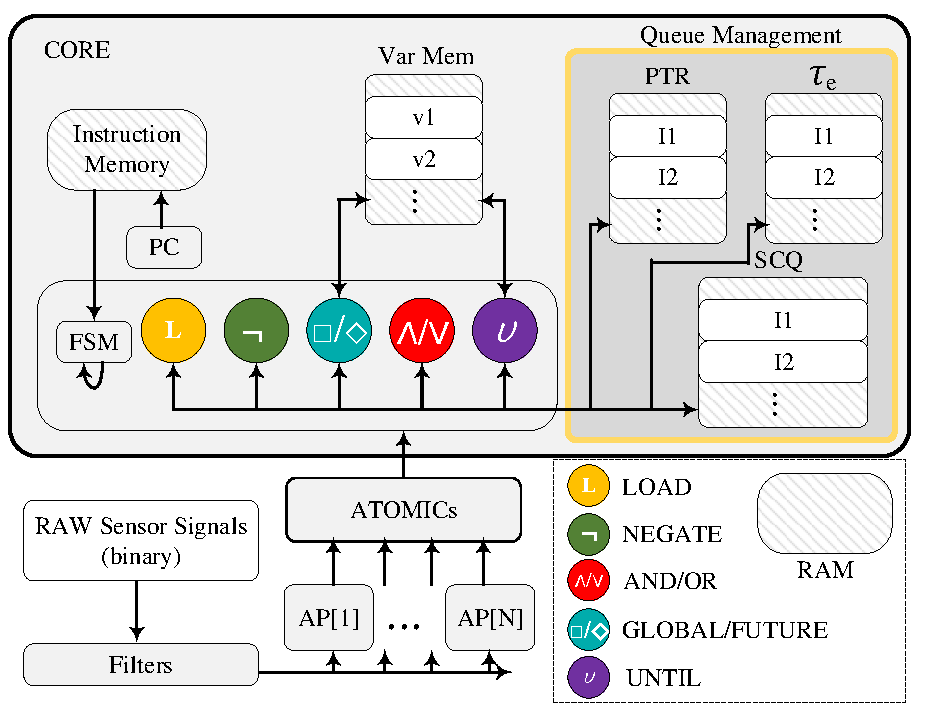
\includegraphics[width=0.55\textwidth]{../fig/core.pdf}
\caption{\label{fig:core}Computation core of the observer.}
\end{figure}

\begin{figure}
\centering
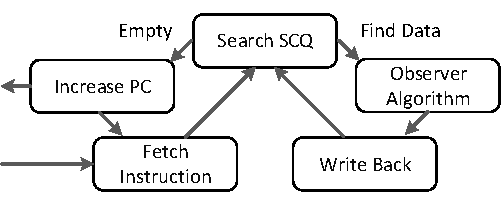
\includegraphics[width=0.55\textwidth]{../fig/wf.pdf}
\caption{\label{fig:wf}State machine transitions of the observer processing core.}
\end{figure}


\section*{Interface for Configuring Hardware Monitor}
We use UART to communicate between FPGA and PC. The PC is used as the 


\section*{Case Study}
\subsection{Verfication on R2}


